\section{Canal RAGB: \texorpdfstring{$M$}{M}-QAM}
\subsection{Modelo}
Considerando que um sinal ($s_m$) de mensagem passa por um canal de Ruído Adivitivo Gaussiano Branco (RAGB), o modelo da Equação~\ref{eq:AWGM_Model}, onde como uma variável aleatoria, $\mathcal{C} \mathcal{N} (0,N_0)$, Gaussiana complexa com média zero e variância $N_0$. 
\begin{equation}
    y_m = s_m + n_m
    \label{eq:AWGM_Model}
\end{equation}

A variância é dada por $\sigma_{n}^{2} = \frac{N_0}{2}$, representando a potência média do ruído que afeta cada dimensão do sinal em banda base~\cite{Proakis}. Consequentemente, o desvio padrão do ruído corresponde a $\sqrt{\frac{N_0}{2}}$, poderando parte real e imaginária. Portanto, tendo um valor de SNR ($E_s\_N_0$) em dB, o termo $N_0$ pode ser calculado por $N_0= E_s 10^{-\frac{E_s\_N_0}{10}}$, tendo enfim o termo $n_m$ é obtido na equação~\ref{eq:termo_ruido}.
\begin{equation}
    n_m = \sqrt{\frac{N_0}{2}} \left(\text{randn}(1) + 1j \text{randn}(1)\right)
    \label{eq:termo_ruido}
\end{equation}

Para ilustrar a implementação do modelo, as constelações $M$-QAM recebem uma sequência de símbolos com SNR de 25dB gerados no script \href{https://raw.githubusercontent.com/lucasabdalah/Courses-HWs/SCD/Sistemas%20de%20Comunicacoes%20Digitais/matlab/problema3/script_AWGN.m}{\colorbox{gray!10}{\color{red}script\_AWGN.m}}, como mostrado na figura~\ref{fig:4QAM_25dB}, \ref{fig:16QAM_25dB} e \ref{fig:64QAM_25dB}.

\begin{figure}[!ht]
    \centering
    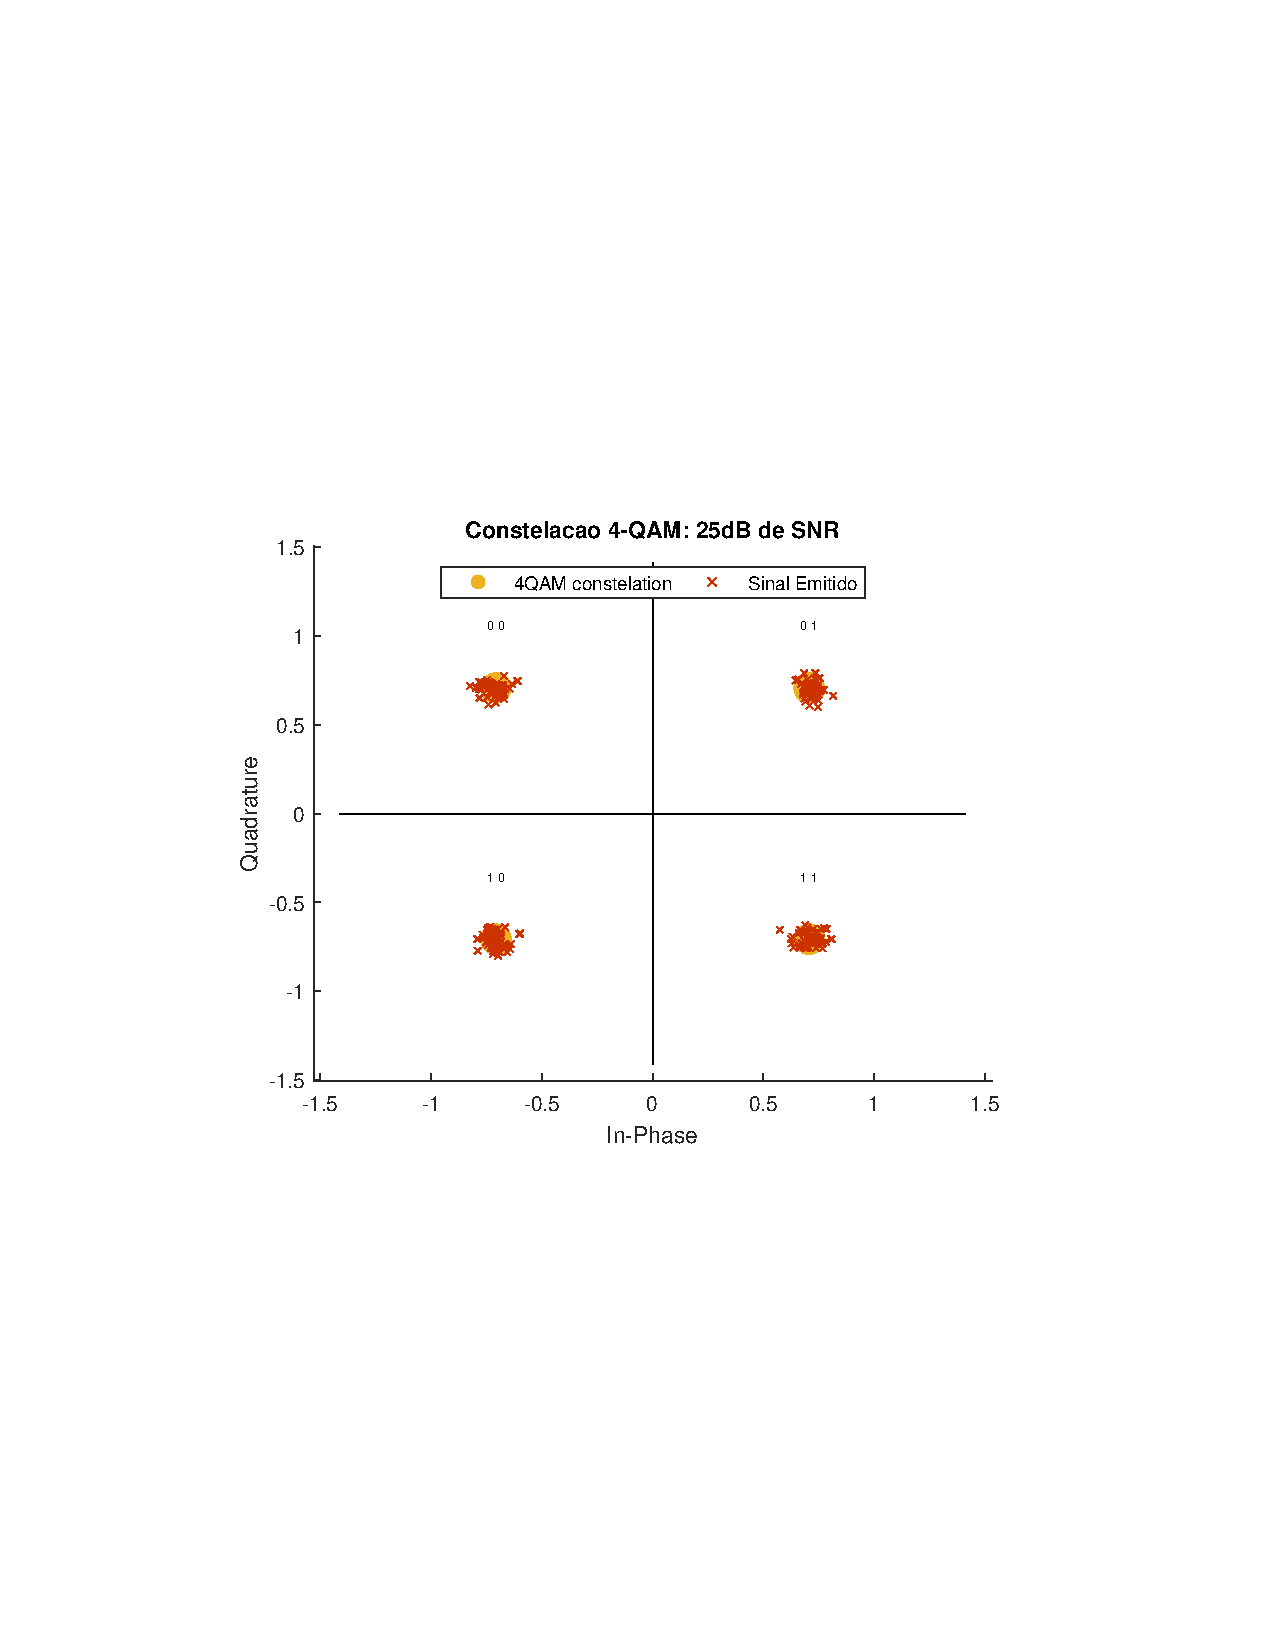
\includegraphics[width=1.0\textwidth,clip=true,trim={1.5cm 8.5cm 1.8cm 8.3cm}]{C:/Users/lukin/Documents/GitHub/Courses-HWs/Sistemas de Comunicacoes Digitais/matlab/problema3/fig/4QAM_25dB.pdf}
    \caption{Simulação de transmissão $4$-QAM, com \textit{SNR} de 25dB.}
    \label{fig:4QAM_25dB}
\end{figure}

\begin{figure}[!ht]
    \centering
    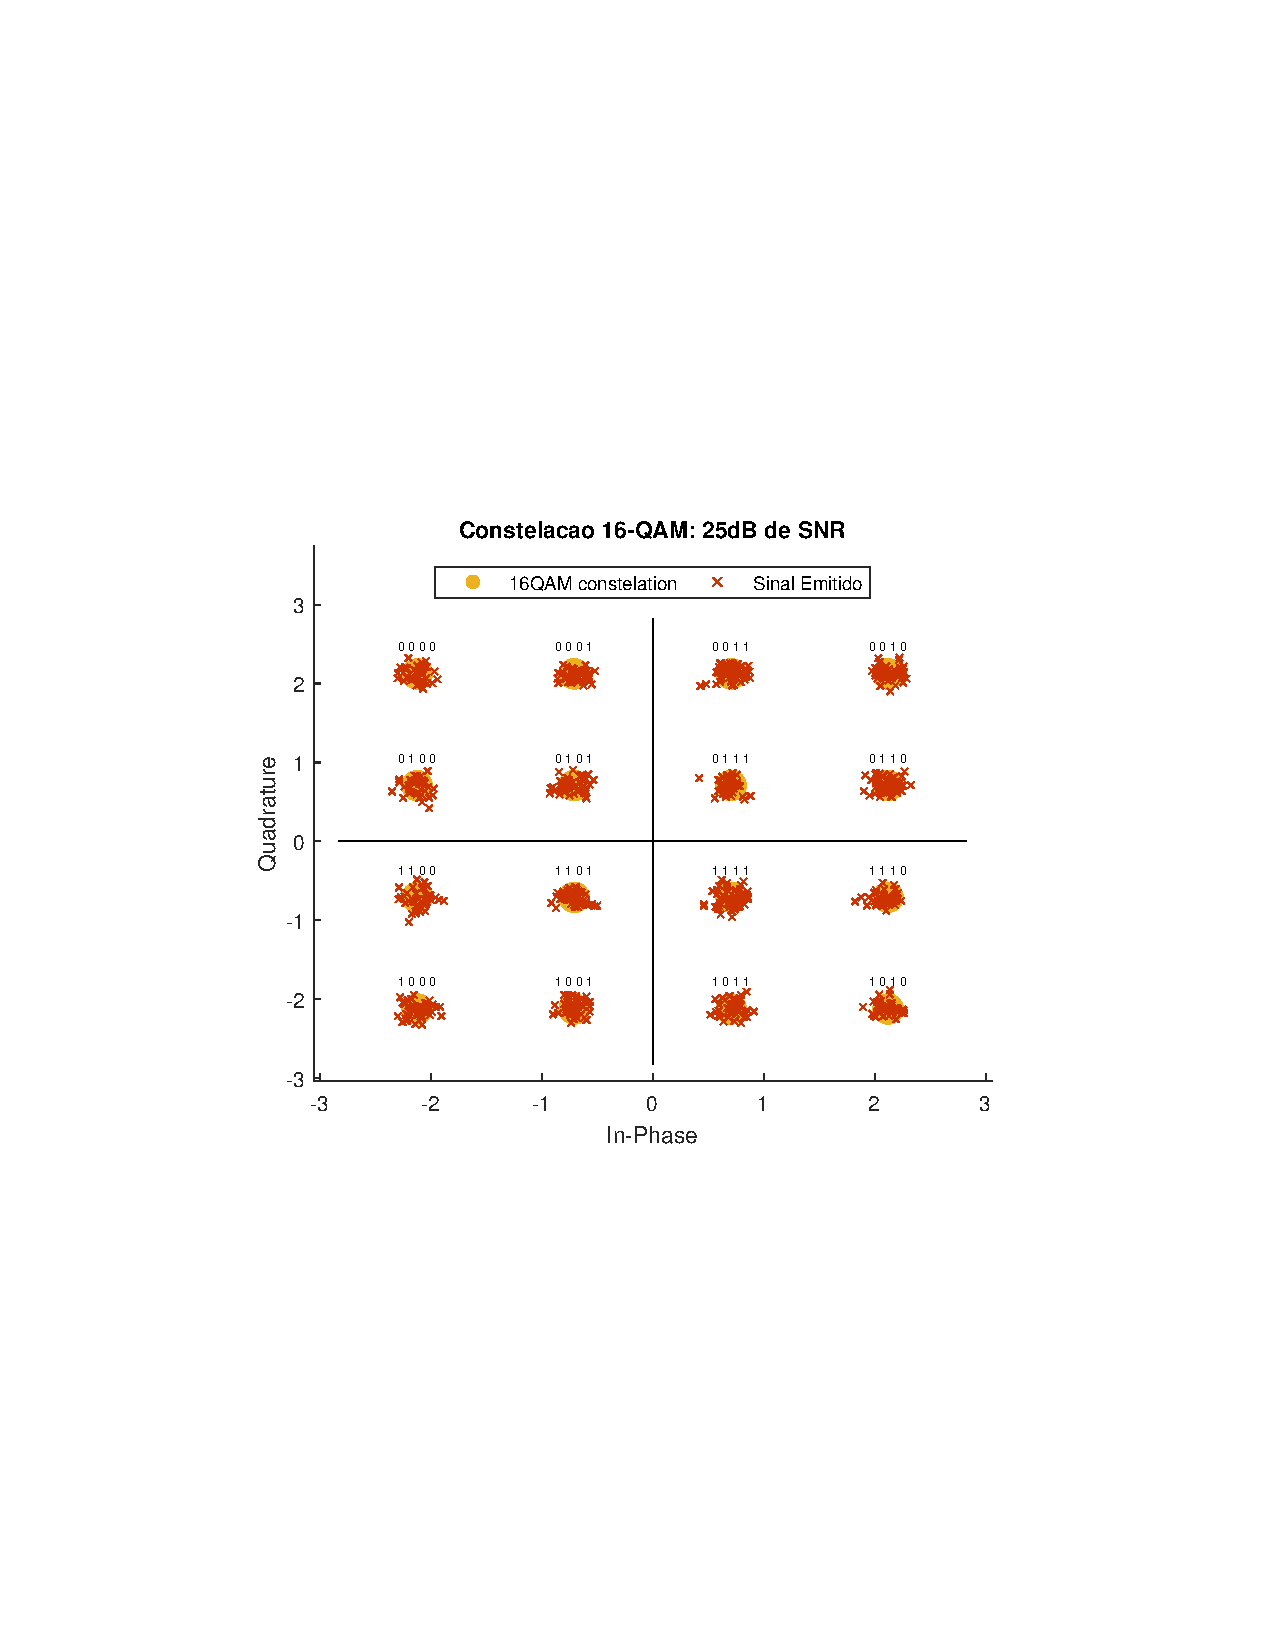
\includegraphics[width=1.0\textwidth,clip=true,trim={1.5cm 8.5cm 1.8cm 8.3cm}]{C:/Users/lukin/Documents/GitHub/Courses-HWs/Sistemas de Comunicacoes Digitais/matlab/problema3/fig/16QAM_25dB.pdf}
    \caption{Simulação de transmissão $16$-QAM, com \textit{SNR} de 25dB.}
    \label{fig:16QAM_25dB}
\end{figure}

\begin{figure}[!ht]
    \centering
    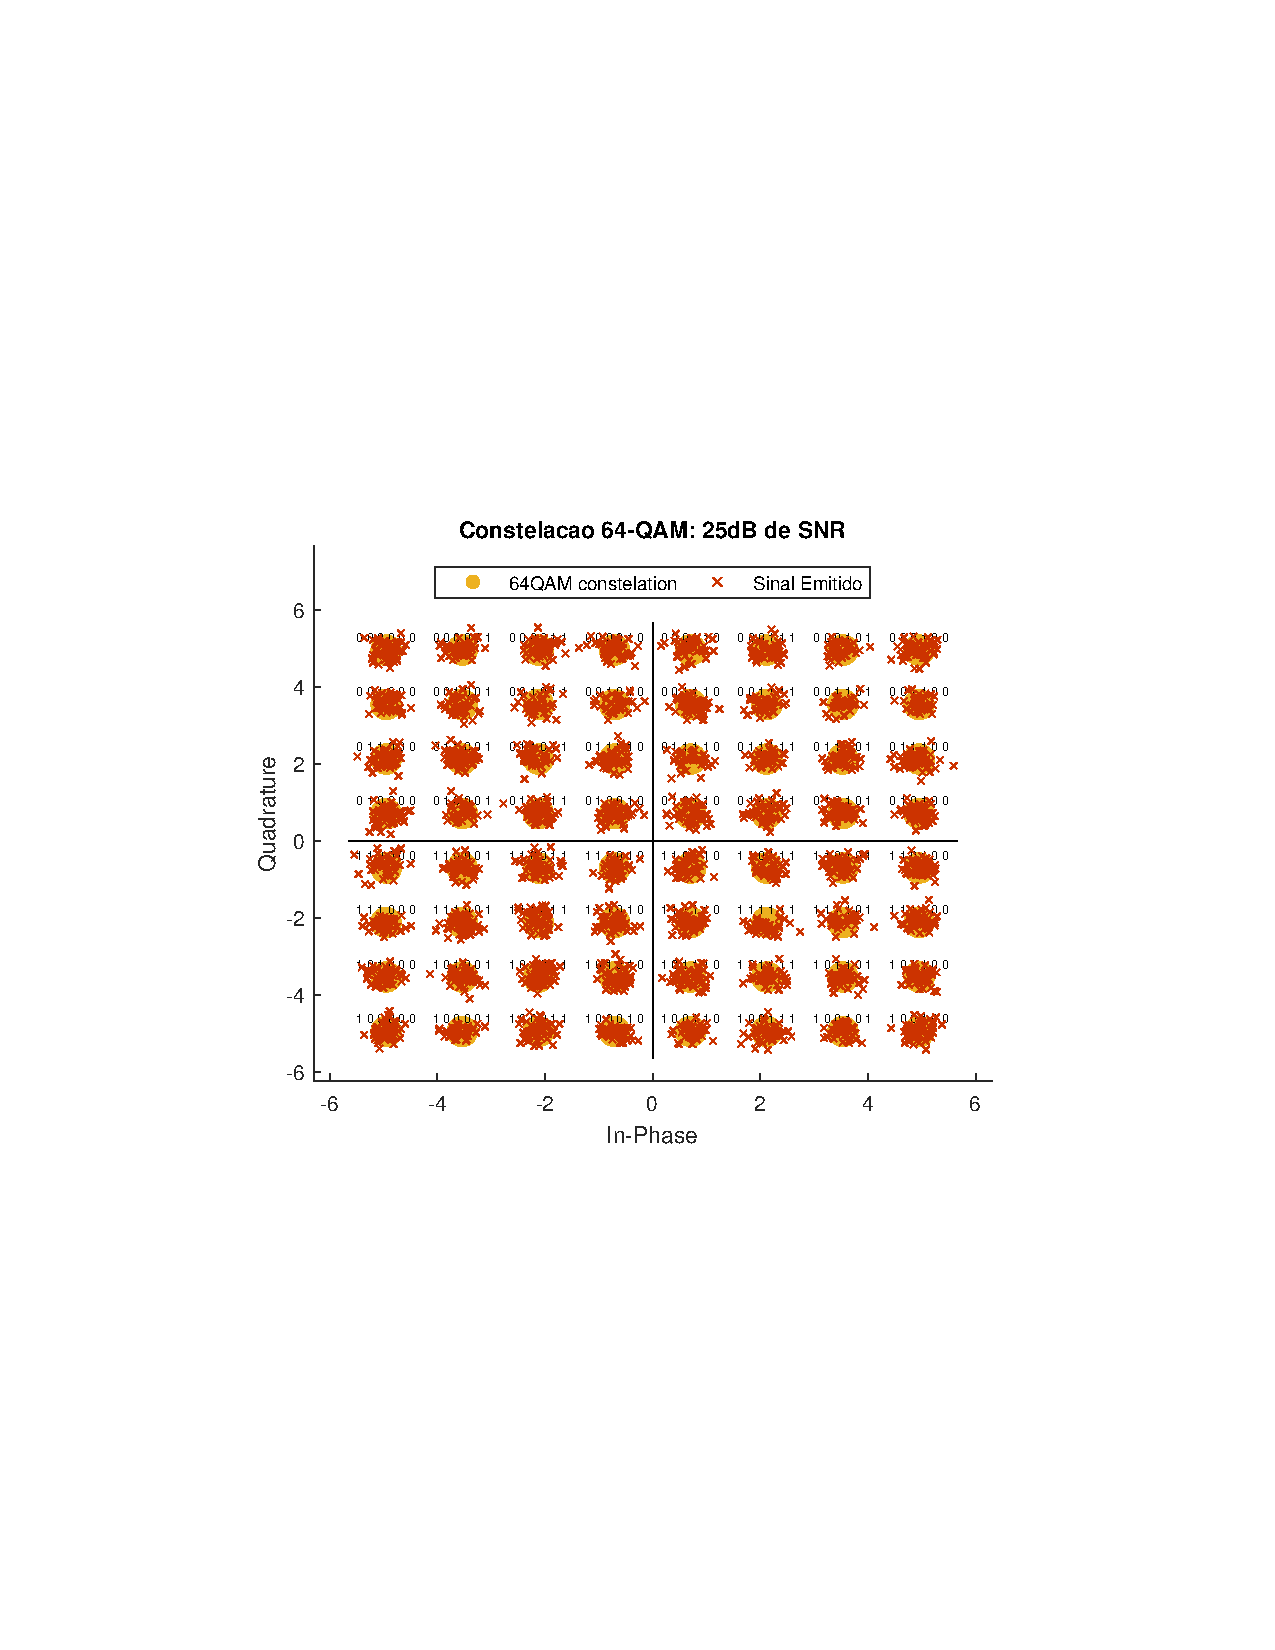
\includegraphics[width=1.0\textwidth,clip=true,trim={1.5cm 8.5cm 1.8cm 8.3cm}]{C:/Users/lukin/Documents/GitHub/Courses-HWs/Sistemas de Comunicacoes Digitais/matlab/problema3/fig/64QAM_25dB.pdf}
    \caption{Simulação de transmissão $64$-QAM, com \textit{SNR} de 25dB.}
    \label{fig:64QAM_25dB}
\end{figure}

\clearpage

\subsection{Experimento de Transmissão}

 O experimento consiste em realizar uma transmissão de uma sequência $s_m$ de tamanho $L = 264000 \text{bits}$ pelo modelo do canal RAGB com as constelações $M$-QAM, variando a \textit{SNR} de 0 a 20 dB com passo 2.

Ao traçar as curvas teóricas de probabilidade de erro de símbolo $P(e)$ e a taxa de erro de símbolo \textit{SER} na figura~\ref{fig:Erro_teoricaxAWGN_MQAM} é possível observar que os valores teóricos e simulados são idênticos, corroborando o embasamento desenvolvido nas seções anteriores.

Estes resultados são gerados com a rotina \href{https://raw.githubusercontent.com/lucasabdalah/Courses-HWs/SCD/Sistemas%20de%20Comunicacoes%20Digitais/matlab/problema3/script_teoricaxAWGN.m}{\colorbox{gray!10}{\color{red}script\_teoricaxAWGN.m}}, que chama os dados já computados nas seções anteriores e traça as curvas em um mesmo gráfico.

\begin{figure}[!ht]
    \centering
    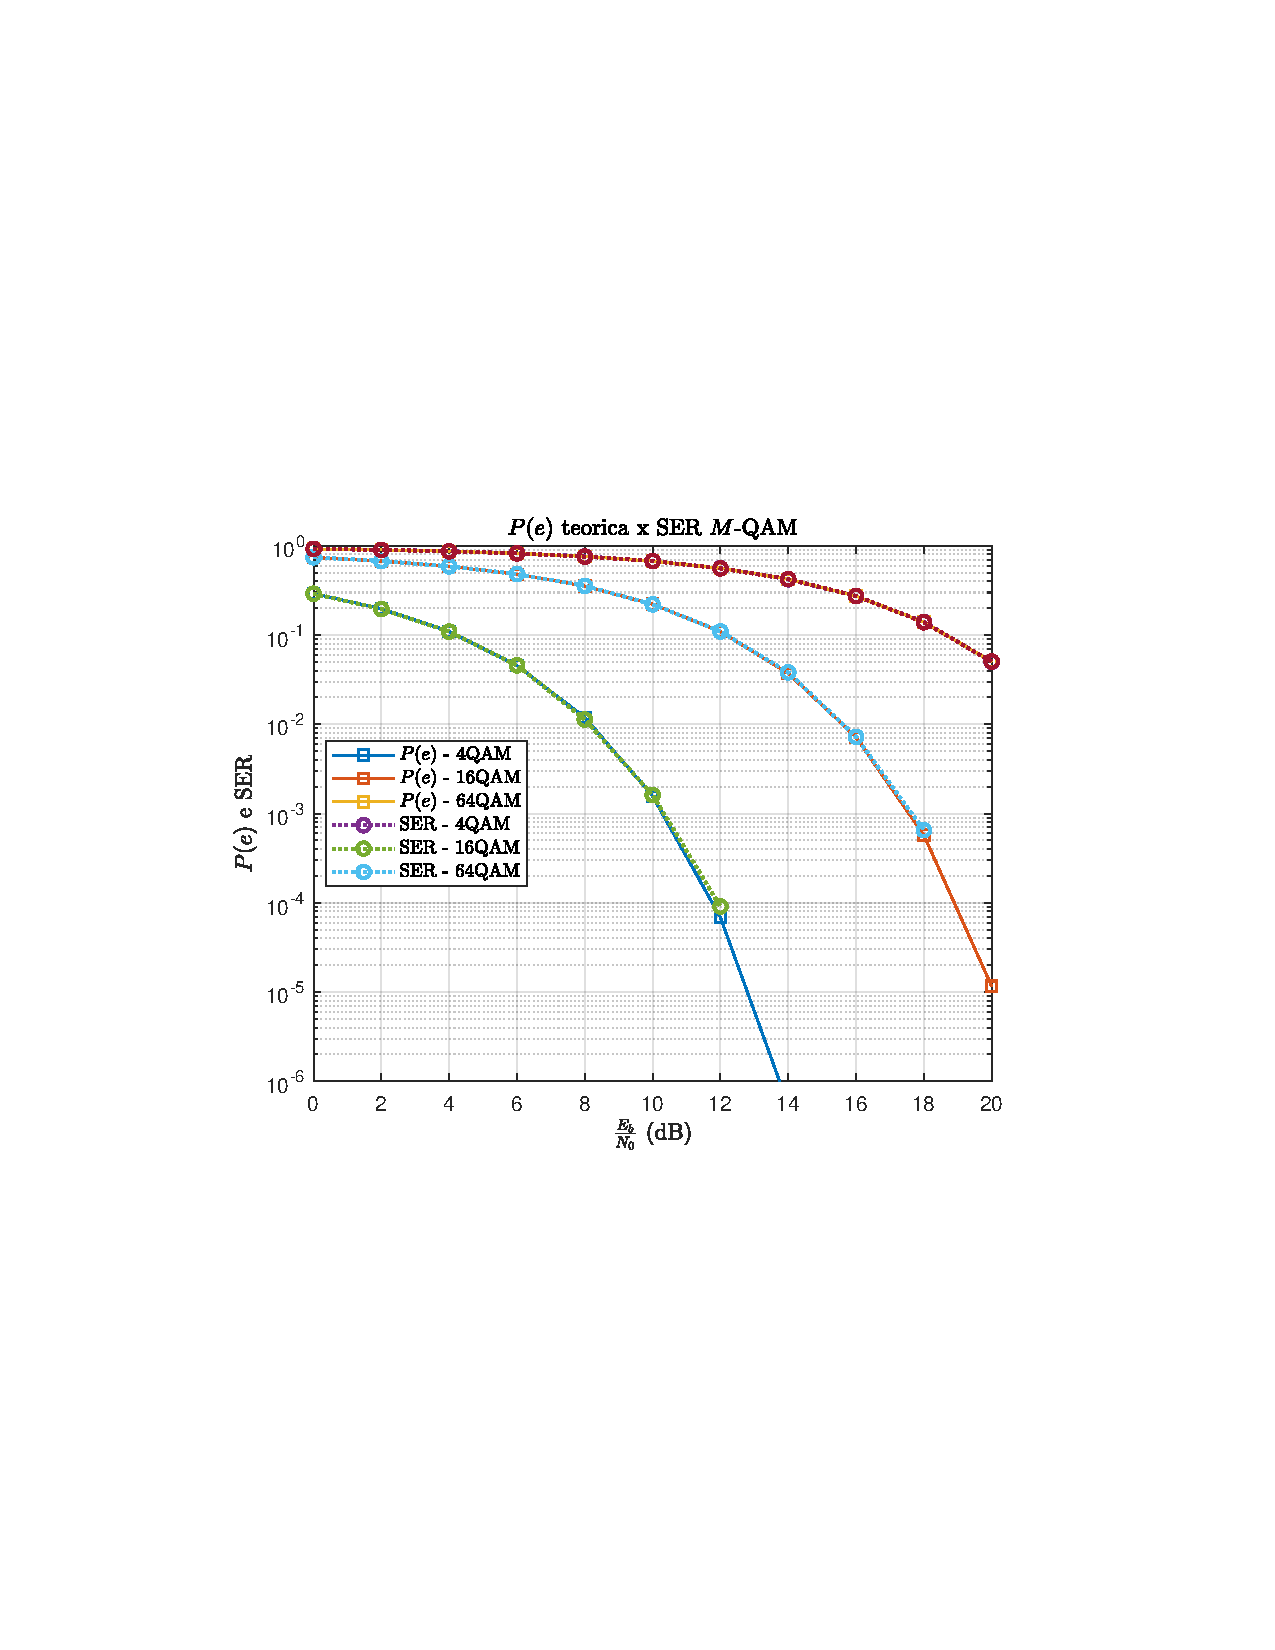
\includegraphics[width=1.0\textwidth,clip=true,trim={1.5cm 8.5cm 1.8cm 8.3cm}]{C:/Users/lukin/Documents/GitHub/Courses-HWs/Sistemas de Comunicacoes Digitais/matlab/problema3/fig/Erro_teoricaxAWGN_MQAM.pdf}
    \caption{Probabilidade teórica de erro vs. simulação de transmissão $M$-QAM em canal RAGB.}
    \label{fig:Erro_teoricaxAWGN_MQAM}
\end{figure}